\documentclass[11pt,a4paper]{article}

\usepackage[utf8]{inputenc}
\usepackage[T1]{fontenc}
\usepackage[english]{babel}
\usepackage{lmodern}
\usepackage{geometry}
\geometry{top=2.3cm,bottom=2.3cm,left=2.4cm,right=2.4cm,headheight=15pt}
\usepackage{hyperref}
\usepackage{enumitem}
\usepackage{booktabs}
\usepackage{tabularx}
\usepackage{array}
\usepackage{graphicx}
\usepackage{fancyhdr}
\usepackage{tikz}
\usepackage{float}
\usepackage{placeins}
\usepackage{xcolor}
\usepackage{caption}
\usepackage{subcaption}
\usepackage{multirow}
\usepackage{colortbl}
\usetikzlibrary{arrows.meta,positioning,shapes.geometric,calc,fit}

\definecolor{wcblue}{HTML}{176B87}
\definecolor{wcgreen}{HTML}{368A3A}
\definecolor{wclight}{HTML}{F4F7FB}
\definecolor{wcgray}{HTML}{566273}

\hypersetup{
    colorlinks=true,
    linkcolor=wcblue,
    urlcolor=wcblue,
    citecolor=wcblue,
    pdftitle={Weighting Cashier - Final Project Report},
    pdfauthor={Martim Calisto Pinheiro, Igor Braga do Espirito Santo, Luis Carlos Ferreira Freitas}
}

\pagestyle{fancy}
\fancyhf{}
\fancyfoot[C]{\thepage}
\renewcommand{\headrulewidth}{0pt}
\setlist[itemize]{leftmargin=1.4em,itemsep=2pt,topsep=3pt}
\captionsetup{font=small,labelfont=bf}

\newcolumntype{Y}{>{\raggedright\arraybackslash}X}
\newcommand{\statusok}{\textcolor{wcgreen}{\textbf{Implemented}}}
\newcommand{\statusvalidated}{\textcolor{wcgreen}{\textbf{Validated}}}
\newcommand{\blankvalue}[1]{\rule{#1}{0.4pt}}
\newcommand{\blankms}{\blankvalue{1.35cm}\,ms}
\newcommand{\figureplaceholder}[2]{%
    \fbox{\parbox[c][#2][c]{0.92\linewidth}{\centering
    \textbf{Physical validation evidence}\\[0.15cm]
    \texttt{#1}}}%
}

\begin{document}

\begin{titlepage}
    \centering
    \vspace*{2.0cm}

    {\Huge\bfseries Weighting Cashier\par}
    \vspace{0.35cm}
    {\LARGE Final Project Report\par}

    \vspace{1.5cm}

    \IfFileExists{scale.png}{
\includegraphics[width=0.34\textwidth]{scale.png}}{\fbox{\parbox[c][3.4cm][c]{0.34\textwidth}{\centering\Large RFID\\Weighting Cashier}}}

    \vspace{1.7cm}

    {\Large\bfseries Embedded Systems\par}
    \vspace{0.25cm}
    {\large Final Delivery\par}

    \vspace{1.2cm}

    {\large
        Martim Calisto Pinheiro (up202509641)\\[0.25cm]
        Igor Braga do Espirito Santo (up201800173)\\[0.25cm]
        Luis Carlos Ferreira Freitas (up201905767)
    }

    \vfill

    \IfFileExists{fcup.png}{
\includegraphics[height=1.8cm]{fcup.png}}{\textbf{Faculty of Sciences, University of Porto}}

    \vspace{0.45cm}

    {\large\bfseries May 29, 2026\par}
\end{titlepage}

\tableofcontents
\newpage

\section{Description of Goals}

The \textit{Weighting Cashier} project implements a supermarket-like checkout system in which products are identified through RFID and associated with weight measurements. Each cashier station is based on an embedded acquisition node connected to a load cell and an RFID reader. A central Raspberry Pi maintains product and price information, associates a customer's Android application with a selected scale, updates active shopping lists, and archives completed transactions.

The core interaction is as follows. A customer first logs into the Android application and reads the RFID tag attached to a cashier scale. From that point onward, products measured by that scale are routed to the shopping list of the associated customer. When a product reading arrives, the central station retrieves its price rule from the product database, calculates the final line-item price, updates the mobile list in real time, and also updates the general-station view.

The project additionally addresses two product pricing modes:
\begin{itemize}
    \item \textbf{Weight-priced products}, such as fruit, whose final cost depends on the stable measured mass and a price per kilogram.
    \item \textbf{Unit-priced products}, such as a bottled product, whose final cost is fixed per item while a recorded weight may still be retained as acquisition information.
\end{itemize}

When a list is completed, the smartphone issues a checkout/reset command. The Raspberry Pi moves that list into an archived receipt record and creates a new empty active session for that customer.

\section{Requirement Analysis}

\subsection{Functional Requirements}

The implemented system satisfies the functional behaviour required for the Weighting Cashier project. The Raspberry Pi central station coordinates two cashier nodes and two Android clients, while keeping product pricing, active lists and archived purchases in a central database.

\begin{tabularx}{\textwidth}{@{}p{0.26\textwidth}Y p{0.18\textwidth}@{}}
\toprule
\textbf{Requirement} & \textbf{Implemented Behaviour and Validation Evidence} & \textbf{Result} \\
\midrule
Product RFID identification & Each cashier node reads a product identifier and transmits it to the Raspberry Pi, where it is resolved through the product database. & \statusvalidated \\
Weight acquisition & Each scale reports product mass through its load-cell acquisition chain. For weight-priced items, pricing is completed only after a valid measured weight is available. & \statusvalidated \\
Price calculation & The central database stores both kilogram-based and fixed unit-based price rules; the server calculates and distributes the correct line-item price. & \statusvalidated \\
Android shopping list & The Android application receives real-time cart updates, presents each item's origin scale and pricing information, and maintains the customer's active total. & \statusvalidated \\
Scale selection by Android & A smartphone associates itself with a cashier station by reading that scale's RFID/NFC pairing tag. & \statusvalidated \\
Reset and archive & The checkout/reset action archives the current shopping list as a grouped receipt and starts a new active list. & \statusvalidated \\
General station & The central web console displays catalogue records, customers, scale nodes, active lists, alerts and archived receipts. & \statusvalidated \\
Two scales and two Androids & Simultaneous station-to-customer routing isolates both sessions, allowing each smartphone to receive only the list generated by its assigned scale. & \statusvalidated \\
\bottomrule
\end{tabularx}
```latex

\subsection{Non-Functional Requirements}

The final integrated assembly was evaluated against the required response-time, concurrency and persistence constraints. Table~\ref{tab:nfr-summary} presents the compliance status of each non-functional requirement, while the detailed measured values and testing procedure are presented in Section~\ref{sec:analysis-evaluation}.

\begin{table}[H]
\centering
\caption{Non-functional requirement compliance summary.}
\label{tab:nfr-summary}
\begin{tabularx}{\textwidth}{@{}p{0.39\textwidth}p{0.23\textwidth}Y@{}}
\toprule
\textbf{Requirement} & \textbf{Target} & \textbf{Compliance} \\
\midrule
RFID product identification & $< 2$ s & Compliant \\
Weight acquisition and stabilisation & $< 2$ s & Compliant \\
Update on smartphone list & $< 2$ s & Compliant \\
Update on general station & $< 2$ s & Compliant \\
Support for scale/identifier cashiers & At least 2 concurrent nodes & Compliant \\
Support for Android clients & At least 2 concurrent clients & Compliant \\
Session preservation and archive & Persistent active and completed lists & Compliant \\
\bottomrule
\end{tabularx}
\end{table}
```

\section{Modelling and Specification}

\subsection{Actors and Main Use Cases}

\begin{itemize}
    \item \textbf{Customer / Smartphone User:} authenticates in the application, selects a scale by reading its tag, observes the current shopping list and completes the purchase through the reset/checkout action.
    \item \textbf{Cashier Station:} reads product RFID information and weight data, then reports measurements to the central station.
    \item \textbf{General Station Operator:} manages products, customers and scales; monitors active shopping lists; inspects archived receipts and runtime alerts.
\end{itemize}

\subsection{Session and Cart Model}

Each active cart belongs to a customer account rather than exclusively to one scale. A customer may be associated with a scale during acquisition, and each stored line item records the scale that originated it. Consequently, previously acquired products remain in the active cart when the customer later associates with another scale, until the customer explicitly completes and archives the list.

Scale assignment is temporary and is maintained through heartbeat messages. This avoids indefinitely blocking a scale after a disconnected mobile session, while preserving cart contents in the Raspberry Pi database.

\subsection{High-Level System Model}

\begin{figure}[H]
\centering
\resizebox{\textwidth}{!}{%
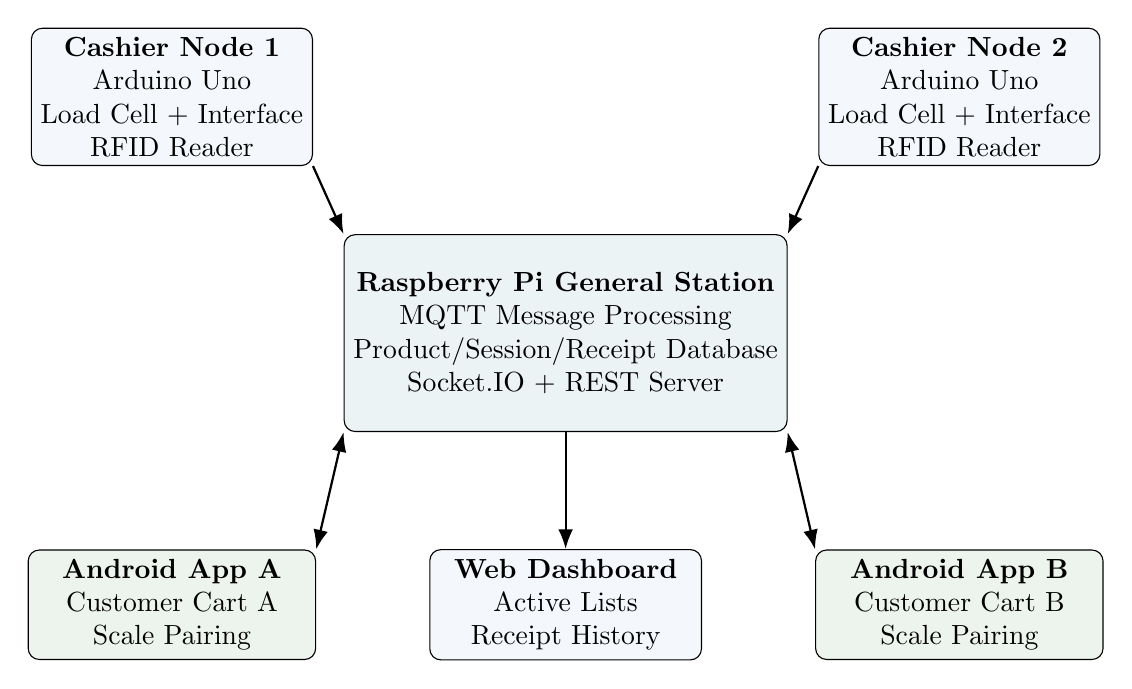
\begin{tikzpicture}[
    box/.style={draw,rounded corners,minimum width=3.45cm,minimum height=1.4cm,align=center,fill=wclight},
    server/.style={draw,rounded corners,minimum width=5.05cm,minimum height=2.5cm,align=center,fill=wcblue!8},
    app/.style={draw,rounded corners,minimum width=3.65cm,minimum height=1.35cm,align=center,fill=wcgreen!9},
    arrow/.style={-{Latex[length=2.5mm]},thick},
    dual/.style={{Latex[length=2.5mm]}-{Latex[length=2.5mm]},thick}
]
\node[box] (scale1) at (0,4.0) {\textbf{Cashier Node 1}\\Arduino Uno\\Load Cell + Interface\\RFID Reader};
\node[box] (scale2) at (10.0,4.0) {\textbf{Cashier Node 2}\\Arduino Uno\\Load Cell + Interface\\RFID Reader};

\node[server] (pi) at (5.0,1.0) {\textbf{Raspberry Pi General Station}\\MQTT Message Processing\\Product/Session/Receipt Database\\Socket.IO + REST Server};

\node[app] (phone1) at (0,-2.45) {\textbf{Android App A}\\Customer Cart A\\Scale Pairing};
\node[box] (admin) at (5.0,-2.45) {\textbf{Web Dashboard}\\Active Lists\\Receipt History};
\node[app] (phone2) at (10.0,-2.45) {\textbf{Android App B}\\Customer Cart B\\Scale Pairing};

\draw[arrow] (scale1.south east) -- (pi.north west);
\draw[arrow] (scale2.south west) -- (pi.north east);

\draw[dual] (phone1.north east) -- (pi.south west);
\draw[dual] (phone2.north west) -- (pi.south east);

\draw[arrow] (pi.south) -- (admin.north);
\end{tikzpicture}%
}
\caption{High-level architecture supporting two cashier nodes and two Android clients. Cashier readings are transmitted through MQTT, while mobile interaction uses REST requests and Socket.IO updates.}
\label{fig:architecture}
\end{figure}

\subsection{Scale Assignment and Product Processing Flow}

\begin{figure}[H]
\centering
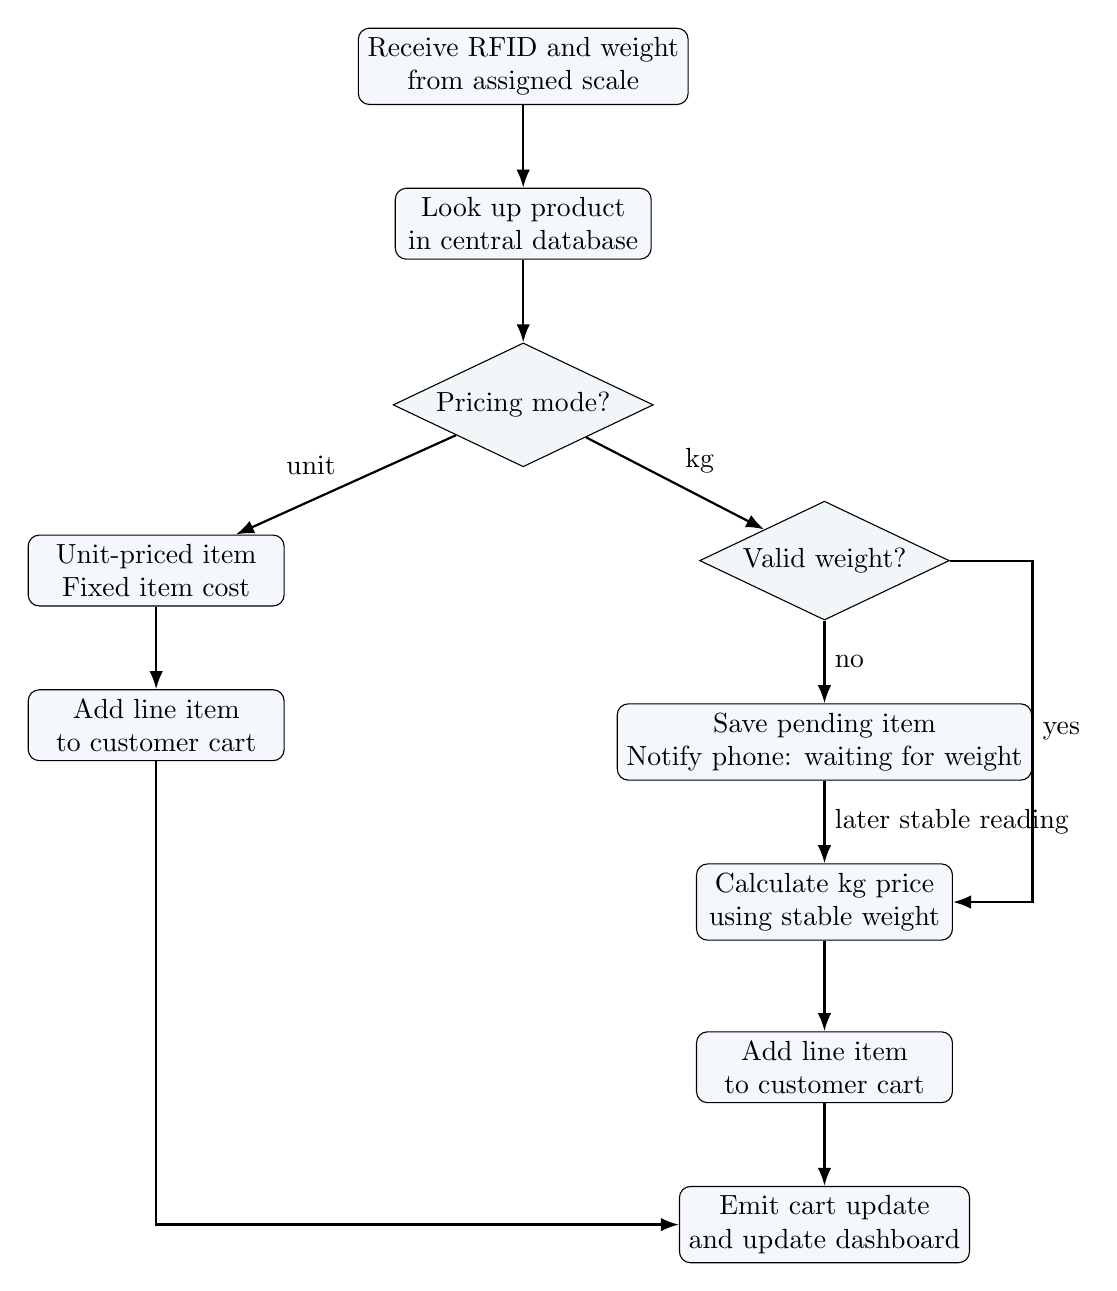
\begin{tikzpicture}[
    node distance=1.05cm and 1.35cm,
    state/.style={draw,rounded corners,minimum width=3.25cm,minimum height=0.82cm,align=center,fill=wclight},
    decision/.style={draw,diamond,aspect=2.1,align=center,inner sep=2pt,fill=wcblue!6},
    arrow/.style={-{Latex[length=2.3mm]},thick}
]
\node[state] (read) {Receive RFID and weight\\from assigned scale};
\node[state, below=of read] (lookup) {Look up product\\in central database};
\node[decision, below=of lookup] (type) {Pricing mode?};
\node[state, below left=1.25cm and 2.2cm of type] (unit) {Unit-priced item\\Fixed item cost};
\node[decision, below right=1.2cm and 2.2cm of type] (valid) {Valid weight?};
\node[state, below=1.05cm of valid] (wait) {Save pending item\\Notify phone: waiting for weight};
\node[state, below=1.05cm of unit] (add1) {Add line item\\to customer cart};
\node[state, below=1.05cm of wait] (calc) {Calculate kg price\\using stable weight};
\node[state, below=1.15cm of calc] (add2) {Add line item\\to customer cart};
\node[state, below=1.05cm of add2] (update) {Emit cart update\\and update dashboard};

\draw[arrow] (read) -- (lookup);
\draw[arrow] (lookup) -- (type);
\draw[arrow] (type) -- node[above left] {unit} (unit);
\draw[arrow] (type) -- node[above right] {kg} (valid);
\draw[arrow] (valid) -- node[right] {no} (wait);
\draw[arrow] (valid.east) -- ++(1.05,0) |- node[pos=0.25,right] {yes} (calc.east);
\draw[arrow] (unit) -- (add1);
\draw[arrow] (wait) -- node[right] {later stable reading} (calc);
\draw[arrow] (calc) -- (add2);
\draw[arrow] (add1.south) |- (update.west);
\draw[arrow] (add2) -- (update);
\end{tikzpicture}
\caption{Server-side treatment of unit-priced and weight-priced products.}
\label{fig:processing}
\end{figure}

\section{Software and Hardware Architecture}

\subsection{Hardware Architecture}

\begin{figure}[H]
\centering
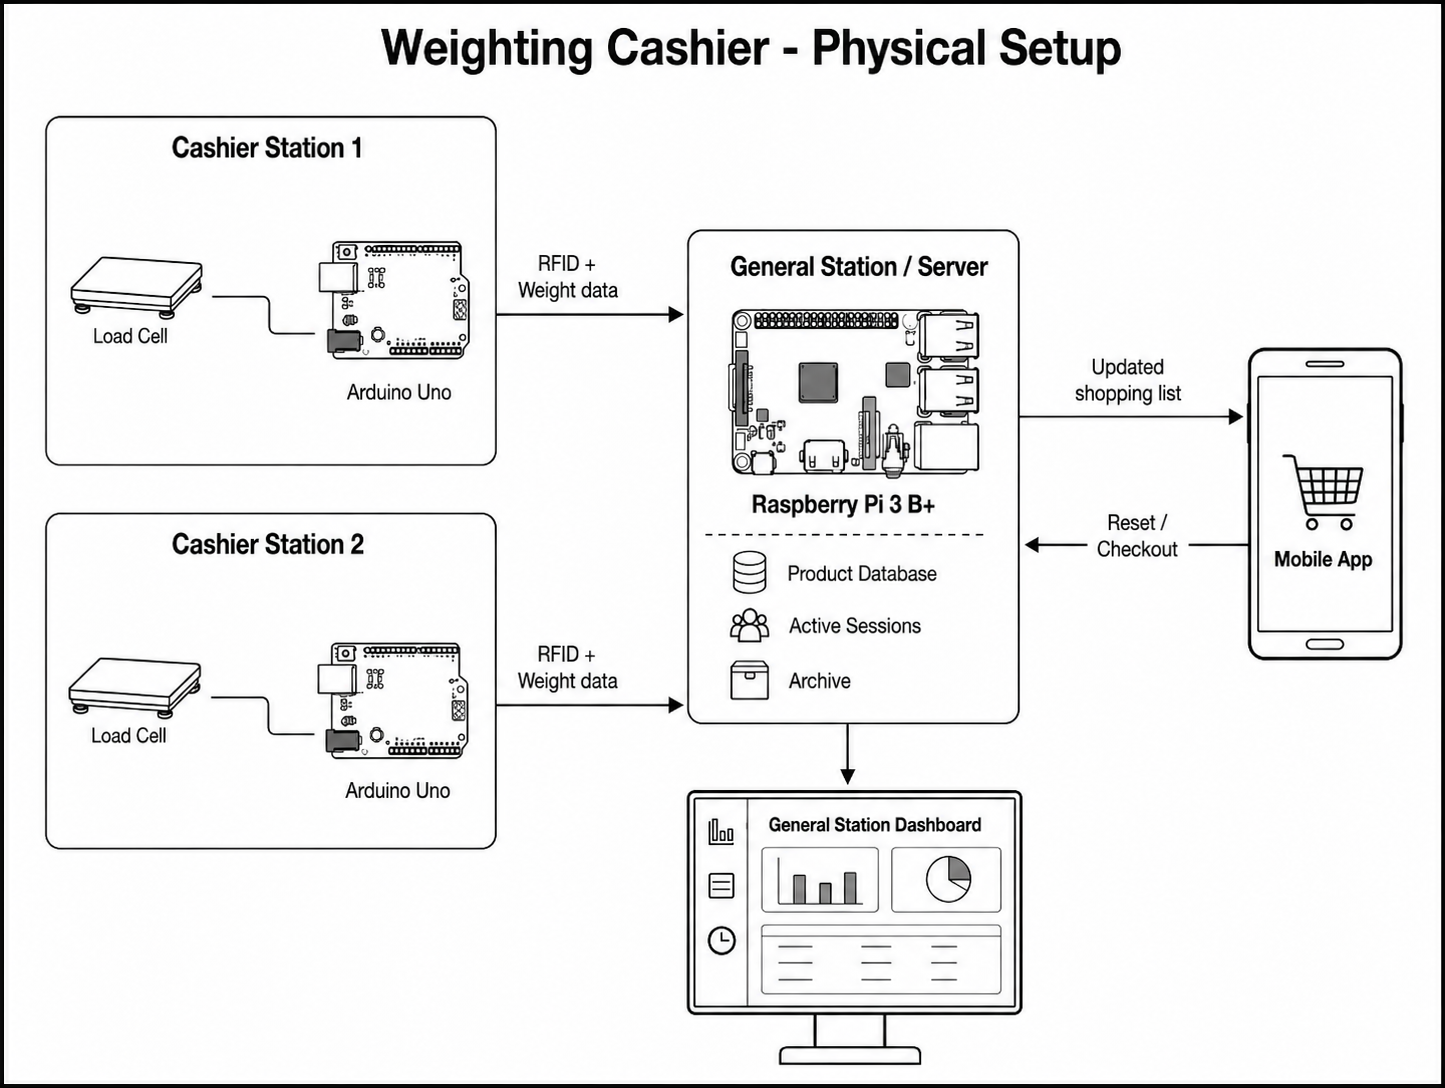
\includegraphics[width=\textwidth]{setupimg.png}
\caption{Physical architecture of the Weighting Cashier system. Each cashier station integrates an Arduino Uno, a load-cell weighing platform, an RFID reader and a communication module. The Raspberry Pi general station manages product data, active sessions and archived purchases, while the Android application displays the shopping list and issues checkout requests.}
\label{fig:physical-architecture-diagram}
\end{figure}



The target physical implementation comprises two independent cashier acquisition nodes and one central station. Each cashier node includes an Arduino Uno, one load cell with its interface/converter module, and one RFID reader. The central station uses a Raspberry Pi to host the server, database, message broker integration and operator dashboard. The Android applications serve as customer interfaces and read the scale-identification tags.

\begin{table}[H]
\centering
\caption{Target hardware components.}
\begin{tabularx}{\textwidth}{@{}p{0.29\textwidth}p{0.16\textwidth}Y@{}}
\toprule
\textbf{Component} & \textbf{Quantity} & \textbf{Purpose} \\
\midrule
Arduino Uno & 2 & Embedded acquisition/control node for each cashier station. \\
Load cell + interface module & 2 + 2 & Measurement of the mass placed on each scale. \\
TinySine NFC Shield v1.0 & 2 & Product RFID/NFC acquisition at each cashier station. \\
RFID/NFC tags & 12 & Identification of products and scale-assignment tags. \\
Network communication module & 2 & Connectivity between each cashier node and the Raspberry Pi server. \\
Raspberry Pi 3 B+ & 1 & General station, application server and persistent database host. \\
Android smartphones & At least 2 & Customer shopping-list interfaces and scale selection. \\
LCD / compatible display setup & 1 & Local development or debug feedback at the general station. \\
Power supplies, USB and wiring & As required & Assembly, power and programming/debug connections. \\
\bottomrule
\end{tabularx}
\end{table}

\subsection{Software Architecture}

\begin{tabularx}{\textwidth}{@{}p{0.27\textwidth}Y@{}}
\toprule
\textbf{Component} & \textbf{Role} \\
\midrule
Android application & Kotlin/Jetpack Compose mobile interface for authentication, NFC scale selection, real-time cart display, checkout and local receipt browsing. \\
Raspberry Pi server & Python server providing REST operations and Socket.IO real-time delivery to customer clients and the operator interface. \\
MQTT communication layer & Event channel between cashier nodes and the central server for readings, tare commands and node status. \\
SQLite database & Stores products and pricing modes, customers, scales, assignments, active carts, readings and archived receipts. \\
General station dashboard & Browser-based interface for catalogue management, scale monitoring, alerts, active carts and expandable receipt history. \\
Mock testing tools & Python scripts representing scale nodes and Android clients for early integration and concurrency tests without physical hardware. \\
\bottomrule
\end{tabularx}


\subsection{Implemented Android Interface}

The Android interface was implemented to support account access, station selection, real-time shopping-list visualisation and receipt consultation. Authentication separates customer sessions before a scale is selected. Once a session is active, the cart interface presents the current accumulated total, connection status, originating scale for each item and the checkout/reset action.

\begin{figure}[H]
\centering
\begin{subfigure}[t]{0.45\textwidth}
    \centering
    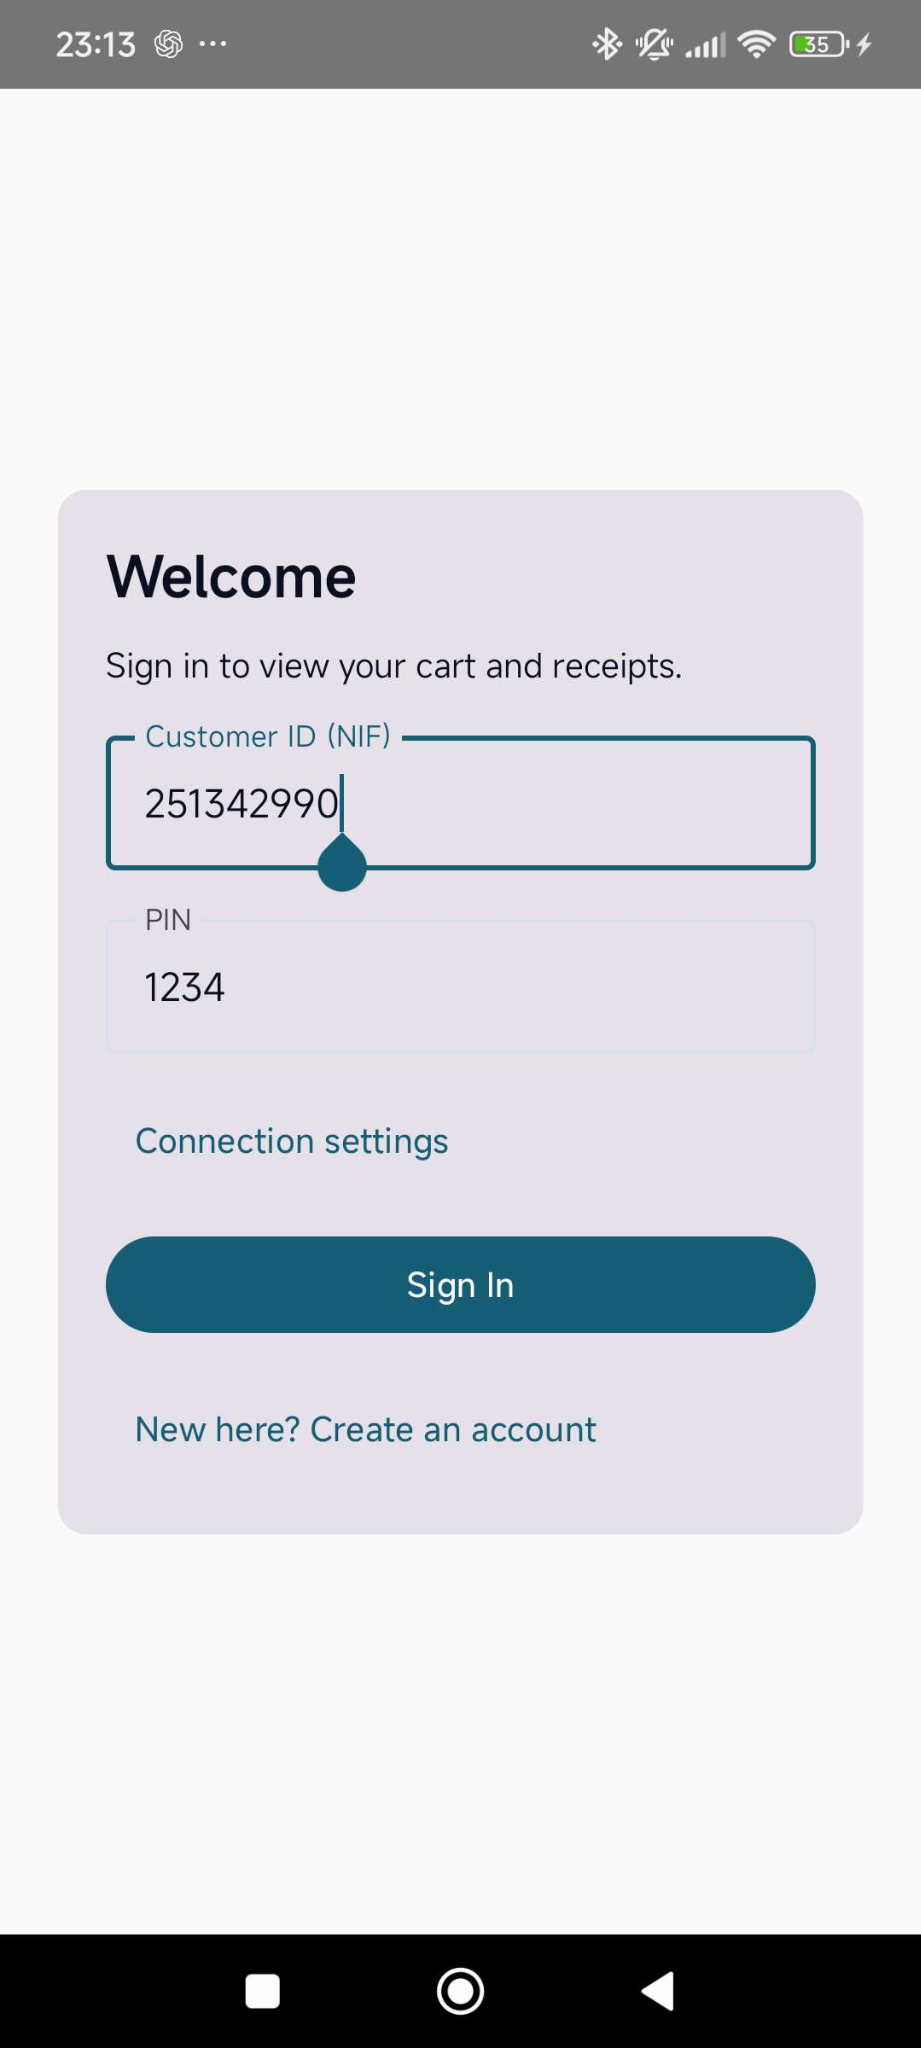
\includegraphics[width=\linewidth]{figures/mobile_login.png}
    \caption{Customer sign-in screen.}
\end{subfigure}
\hfill
\begin{subfigure}[t]{0.45\textwidth}
    \centering
    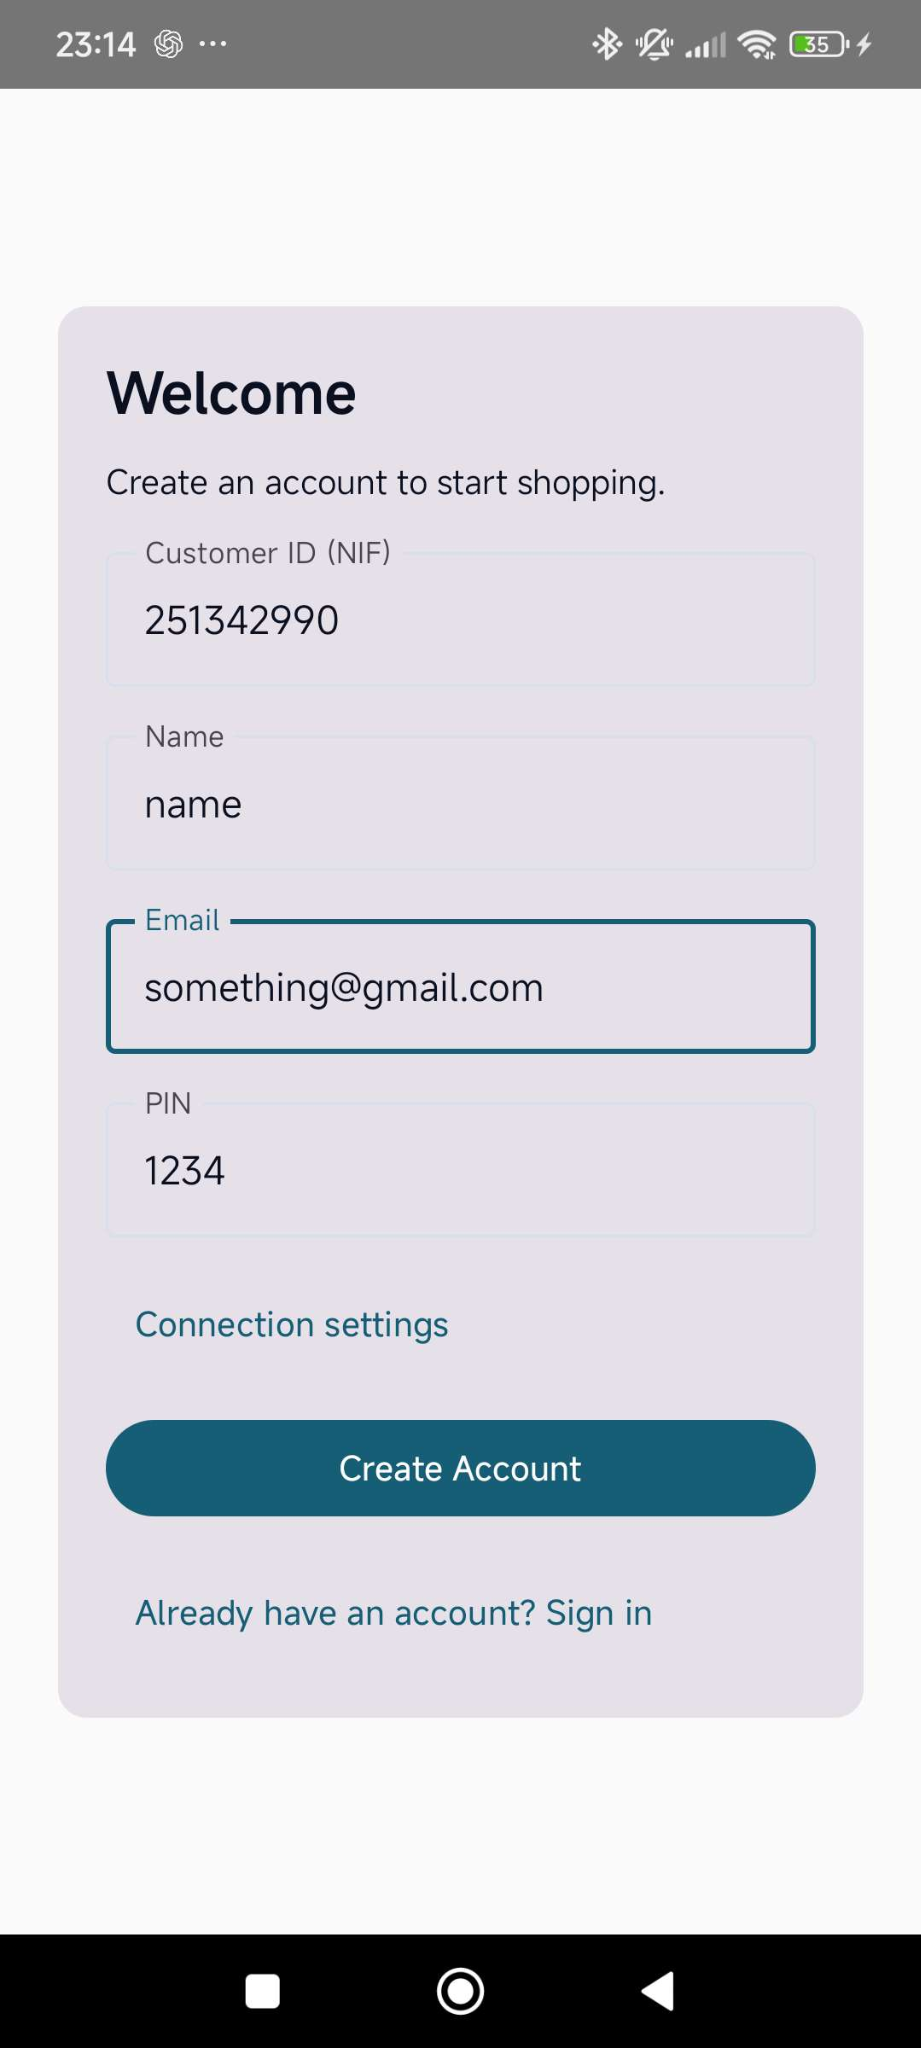
\includegraphics[width=\linewidth]{figures/mobile_registration.png}
    \caption{Account registration screen.}
\end{subfigure}
\caption{Authentication views of the Android mobile application.}
\label{fig:mobile-auth}
\end{figure}

\begin{figure}[H]
\centering
\begin{subfigure}[t]{0.30\textwidth}
    \centering
    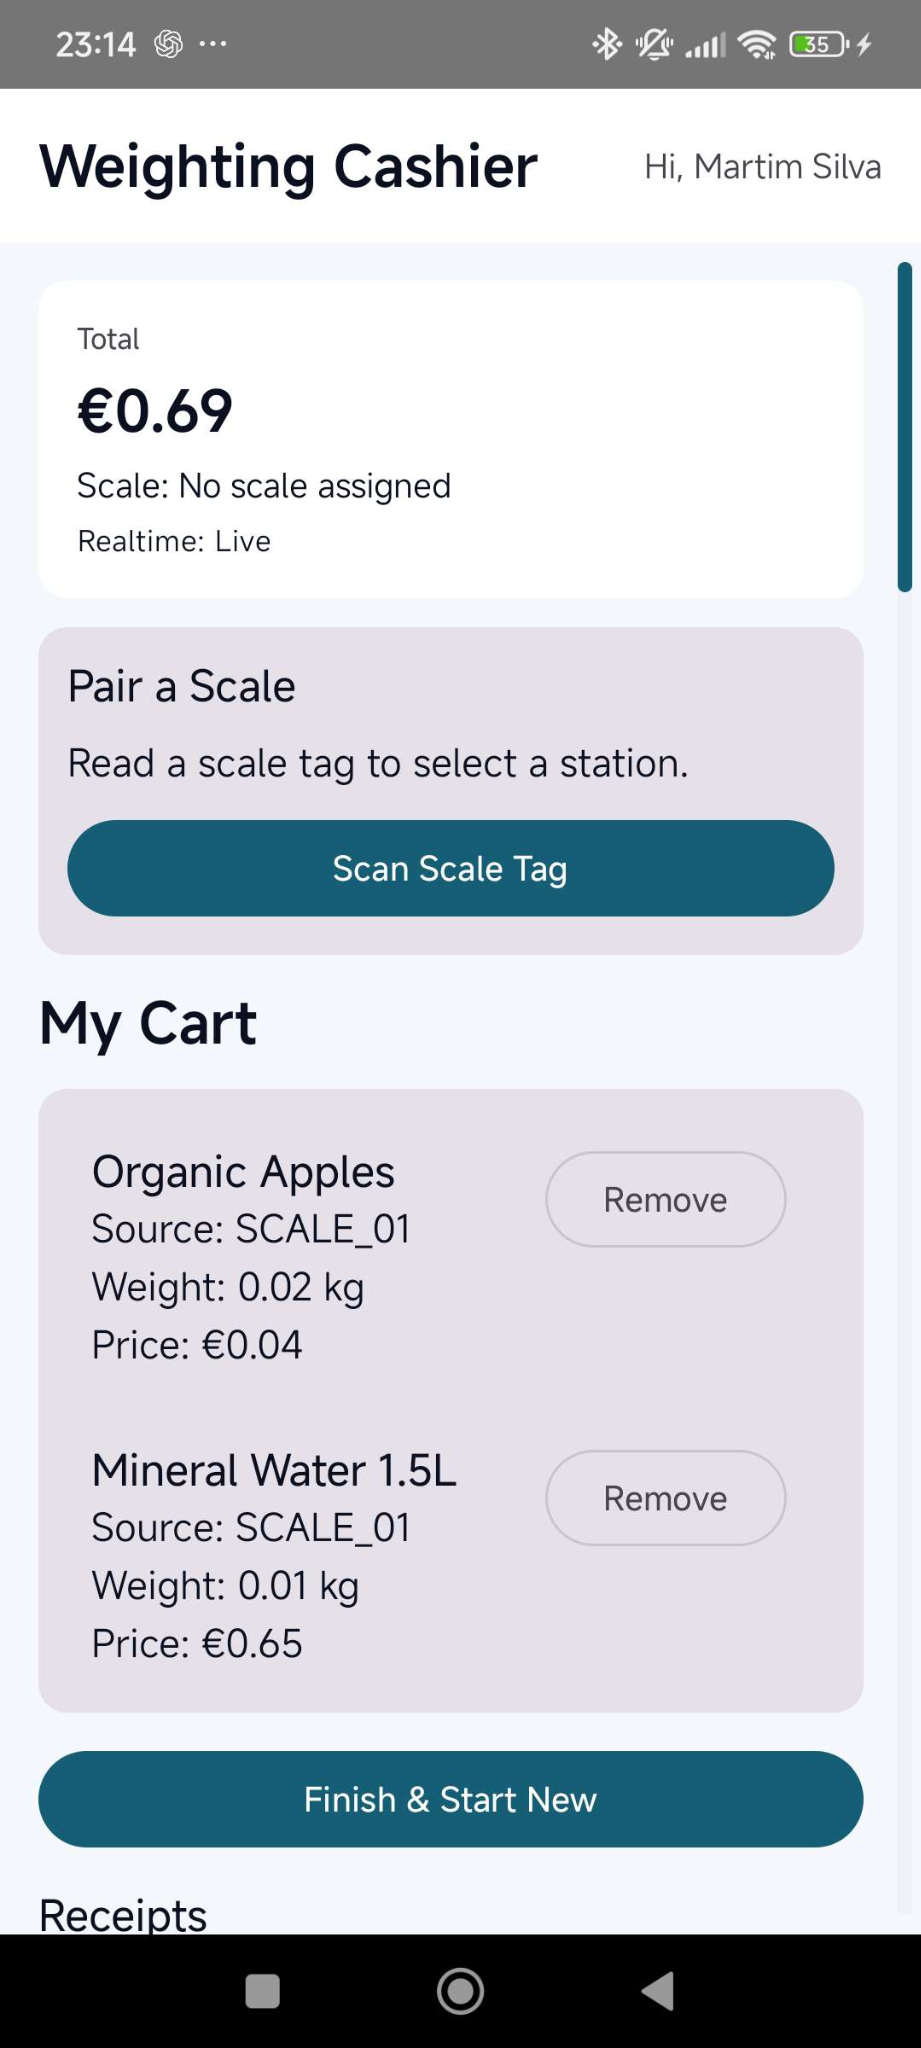
\includegraphics[width=\linewidth]{figures/mobile_cart_overview.png}
    \caption{Current cart and total.}
\end{subfigure}
\hfill
\begin{subfigure}[t]{0.30\textwidth}
    \centering
    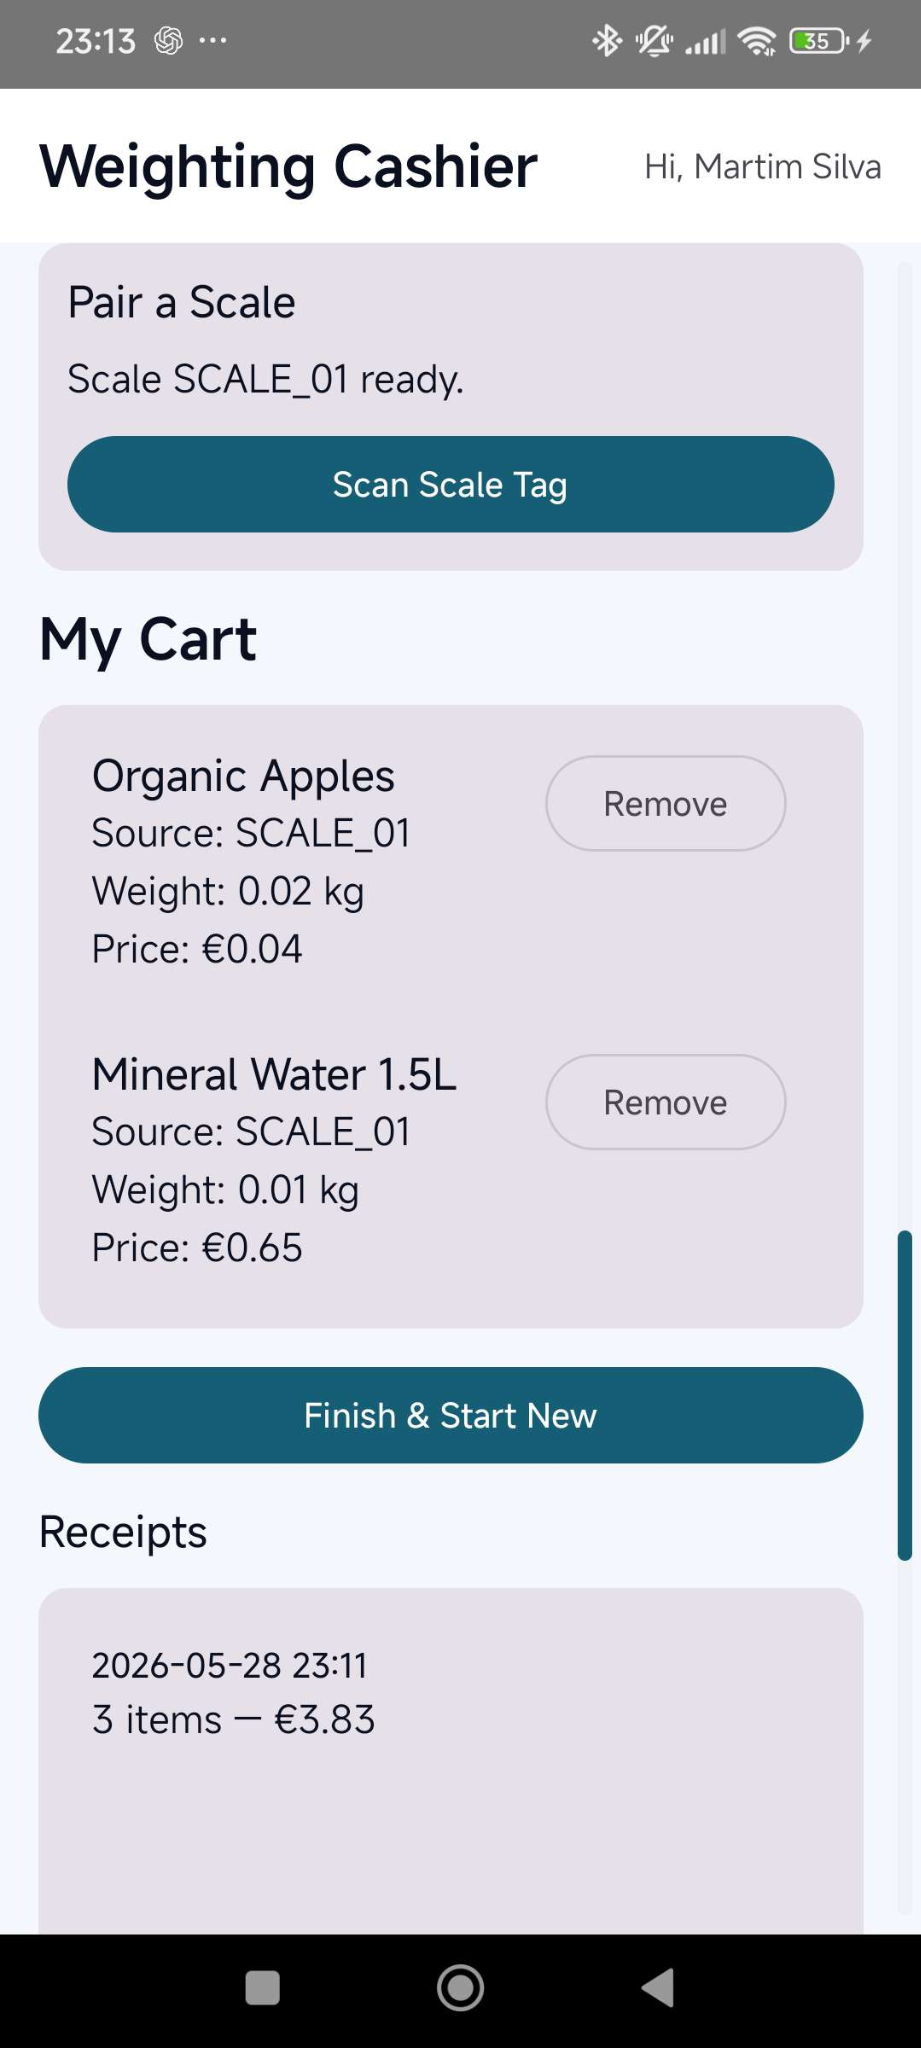
\includegraphics[width=\linewidth]{figures/mobile_cart_and_receipts.png}
    \caption{Paired station and receipts.}
\end{subfigure}
\hfill
\begin{subfigure}[t]{0.30\textwidth}
    \centering
    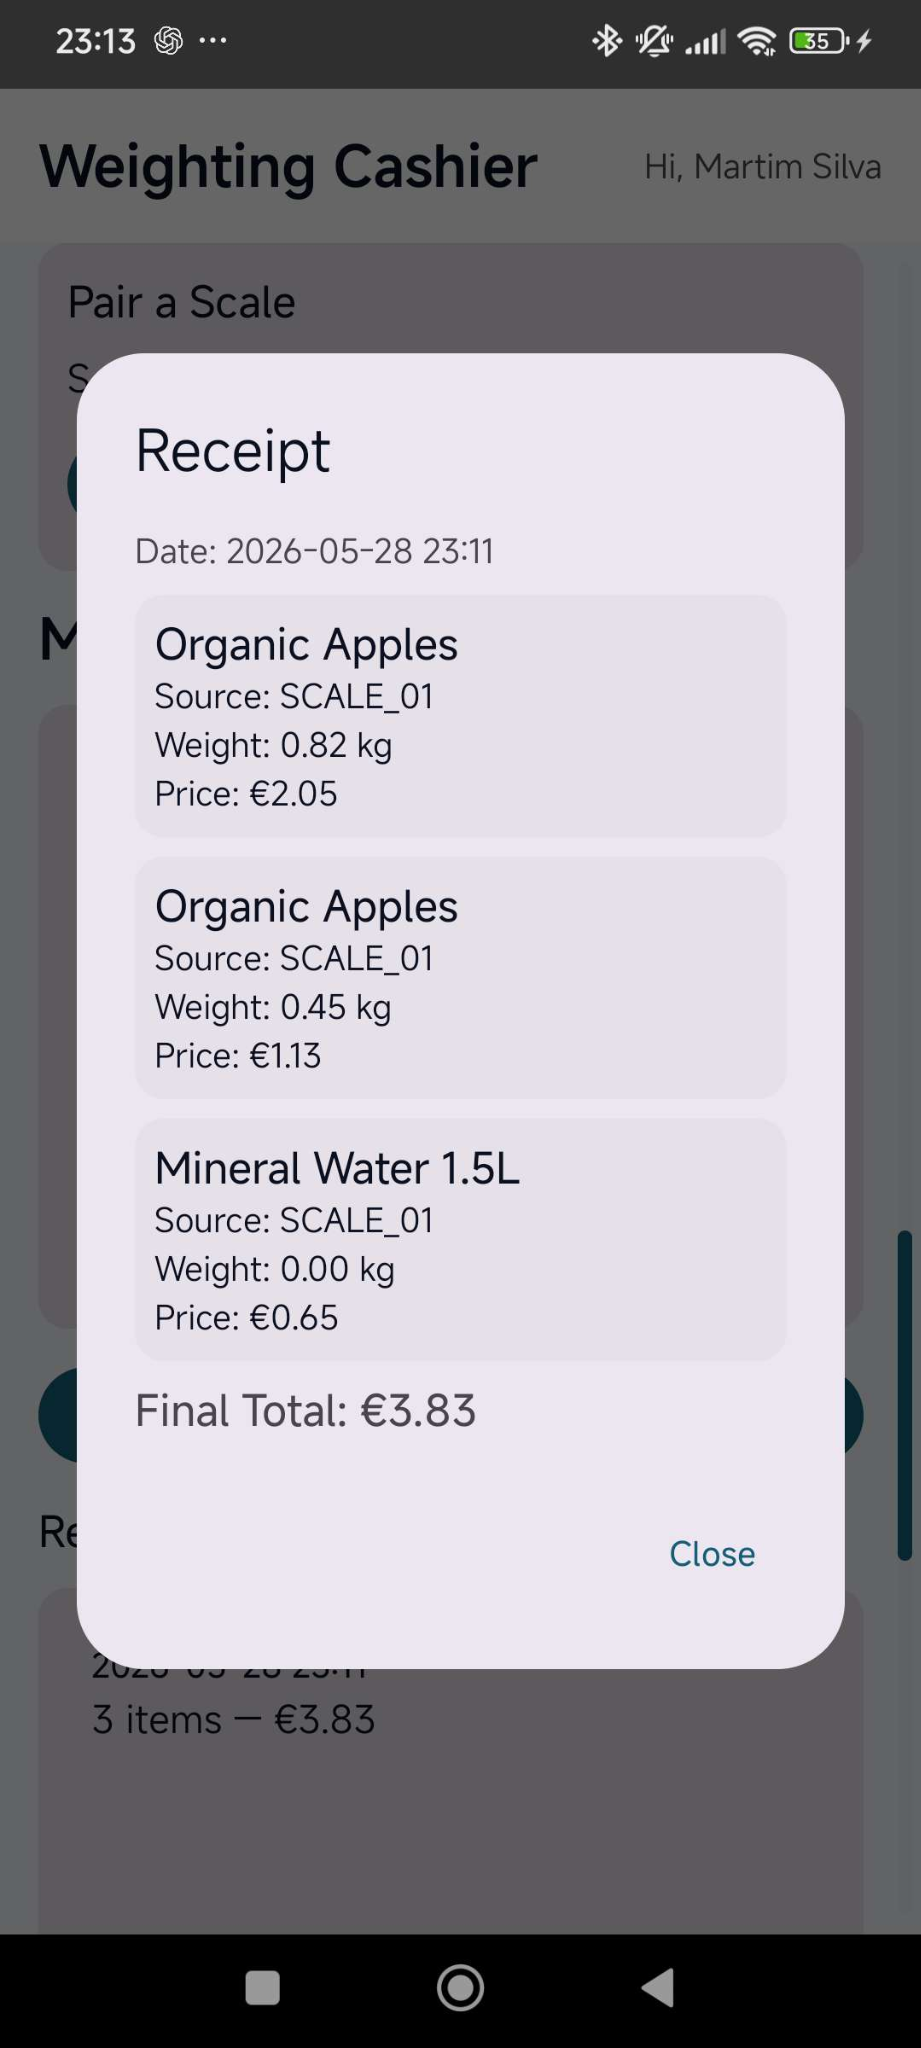
\includegraphics[width=\linewidth]{figures/mobile_receipt_detail.png}
    \caption{Receipt-detail dialog.}
\end{subfigure}
\caption{Implemented shopping-list and archive interaction in the Android application. The screenshots were captured during integration testing; wording of the station-selection panel may be updated in the final interface without altering the underlying workflow.}
\label{fig:mobile-cart}
\end{figure}

\subsection{Interfaces and Data Exchange}

\begin{table}[H]
\centering
\caption{Relevant application interfaces.}
\begin{tabularx}{\textwidth}{@{}p{0.31\textwidth}p{0.19\textwidth}Y@{}}
\toprule
\textbf{Interface / Event} & \textbf{Direction} & \textbf{Purpose} \\
\midrule
\texttt{POST /api/auth/login} & Android $\rightarrow$ Server & Authenticates the customer and issues a session token. \\
\texttt{POST /api/scale/assign} & Android $\rightarrow$ Server & Associates the customer with the scale tag read by the smartphone. \\
\texttt{scale\_ready} & Server $\rightarrow$ Android & Confirms assignment after the scale has completed its tare operation. \\
MQTT \texttt{.../reading} & Scale $\rightarrow$ Server & Delivers product RFID, weight and optional capture timestamp. \\
\texttt{cart\_notice} & Server $\rightarrow$ Android & Communicates pending weight acquisition for a bulk item. \\
\texttt{cart\_update} & Server $\rightarrow$ Android & Transmits the latest shopping-list contents and computed prices. \\
\texttt{POST /api/cart/reset} & Android $\rightarrow$ Server & Archives the active cart as a receipt and starts a new list. \\
\texttt{performance\_event} & Server $\rightarrow$ Client & Reports measured software-pipeline processing timestamps. \\
\bottomrule
\end{tabularx}
\end{table}

\section{Integration}

\subsection{Integrated Operational Flow}

The integrated workflow begins with customer authentication on the Android application. The smartphone identifies the selected scale by reading its tag and submitting the value to the Raspberry Pi. Once the server accepts the requested association, it issues a tare command to the corresponding cashier node and only activates the session after the scale confirms readiness.

After assignment, each product reading originating from that scale is routed to the associated customer's cart. Product identification and price determination are performed centrally. This avoids storing price rules at the cashier nodes and ensures that the mobile application and general station use the same price source.

For kilogram-priced products, a zero or absent mass does not immediately produce a charged line item. Instead, the server stores a temporary pending product state and emits a notice to the mobile application requesting a valid scale reading. Once weight becomes available, the item is priced and added to the cart. For unit-priced items, the fixed item price can be applied immediately, while any acquired weight remains informational.

\subsection{Receipt Archive and General Station}

When the user selects the checkout/reset action in the application, the active list is transferred to the archive. The updated archive design groups line items by receipt identifier, allowing the general-station History interface to display one expandable completed shopping list rather than unrelated product rows. Each receipt records customer identity, scales involved, timestamp, individual pricing rules and final total.

\subsection{General Station Control Panel}

The Raspberry Pi general station exposes an administrative web interface for management and monitoring. The product catalogue stores RFID identifiers and pricing rules, the customer view identifies active application users, and the hardware-nodes panel registers the two scale identifiers and their pairing tags. The History view is designed to display archived shopping lists grouped as completed receipts.

\begin{figure}[H]
\centering
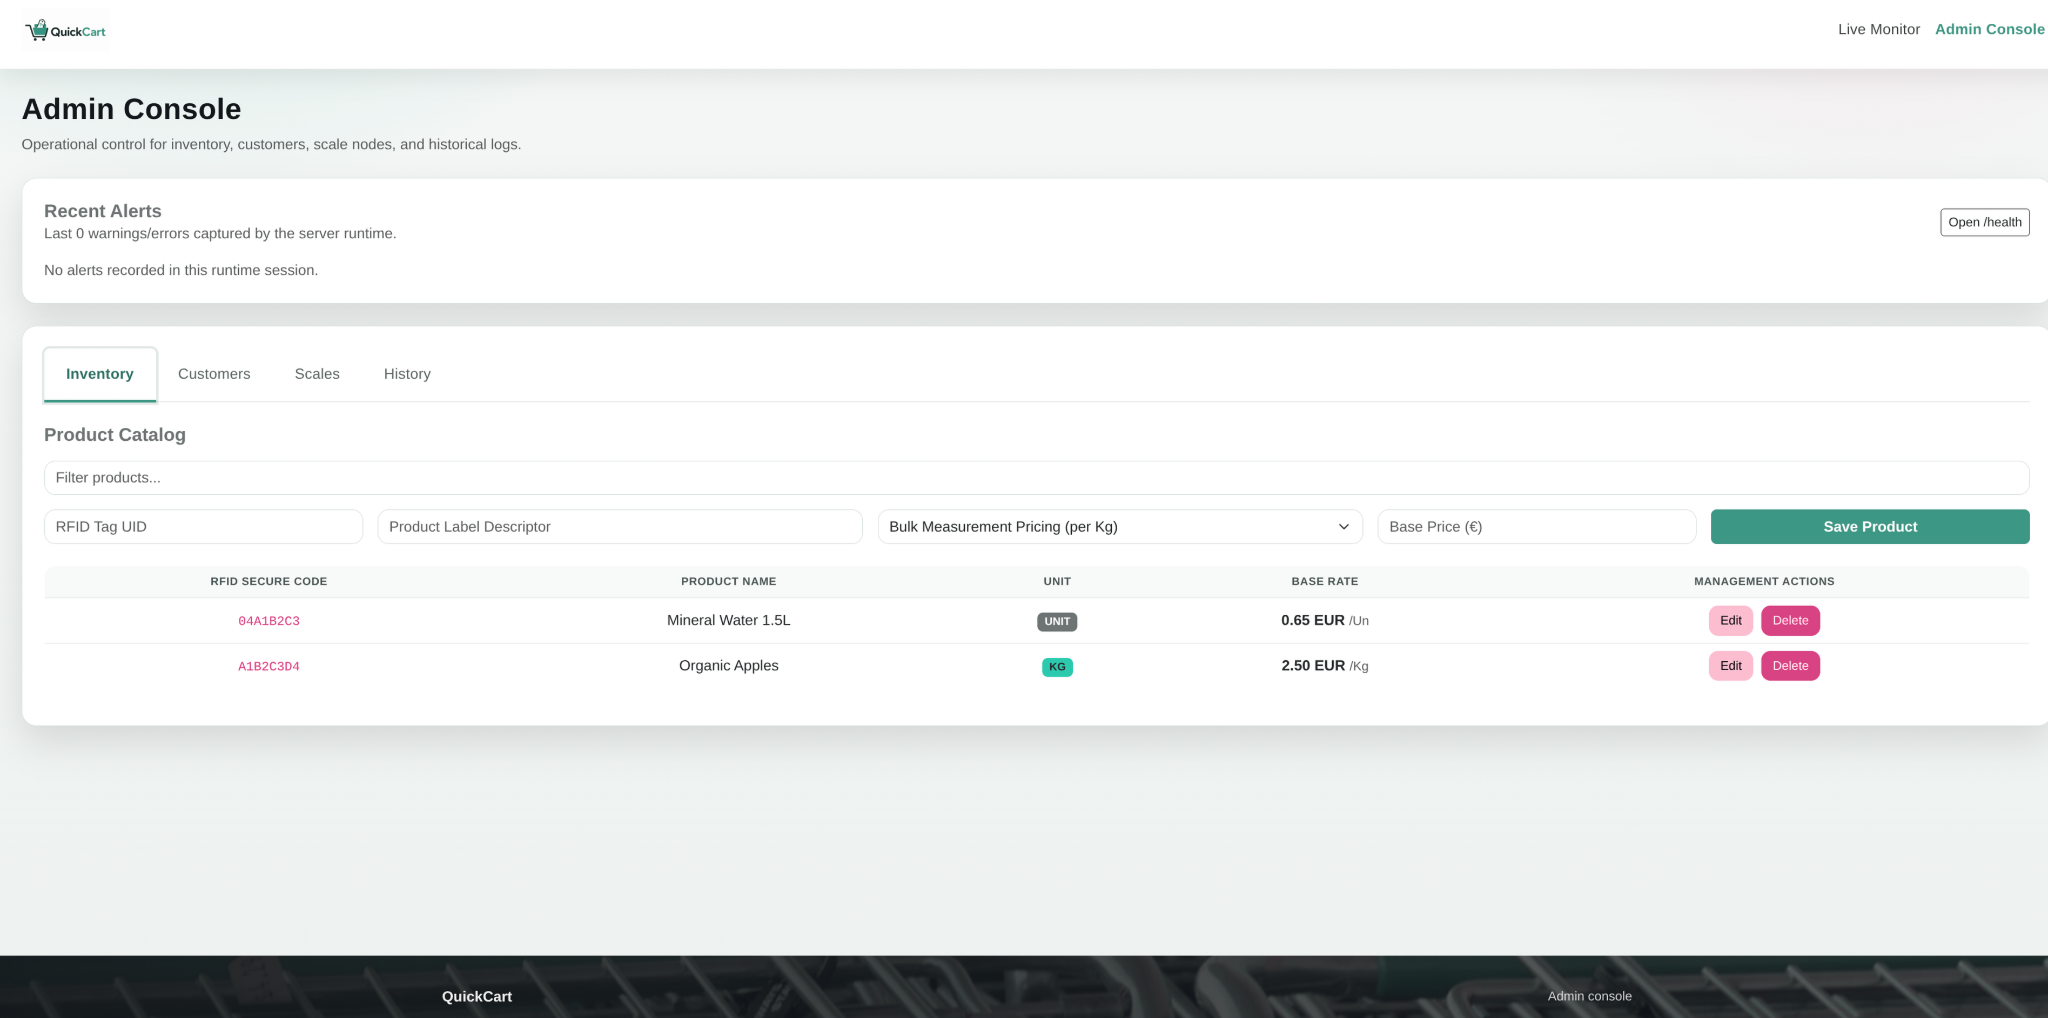
\includegraphics[width=\textwidth]{figures/admin_inventory.png}
\caption{General-station inventory view, including RFID identifiers and price rules.}
\label{fig:admin-inventory}
\end{figure}

\begin{figure}[H]
\centering
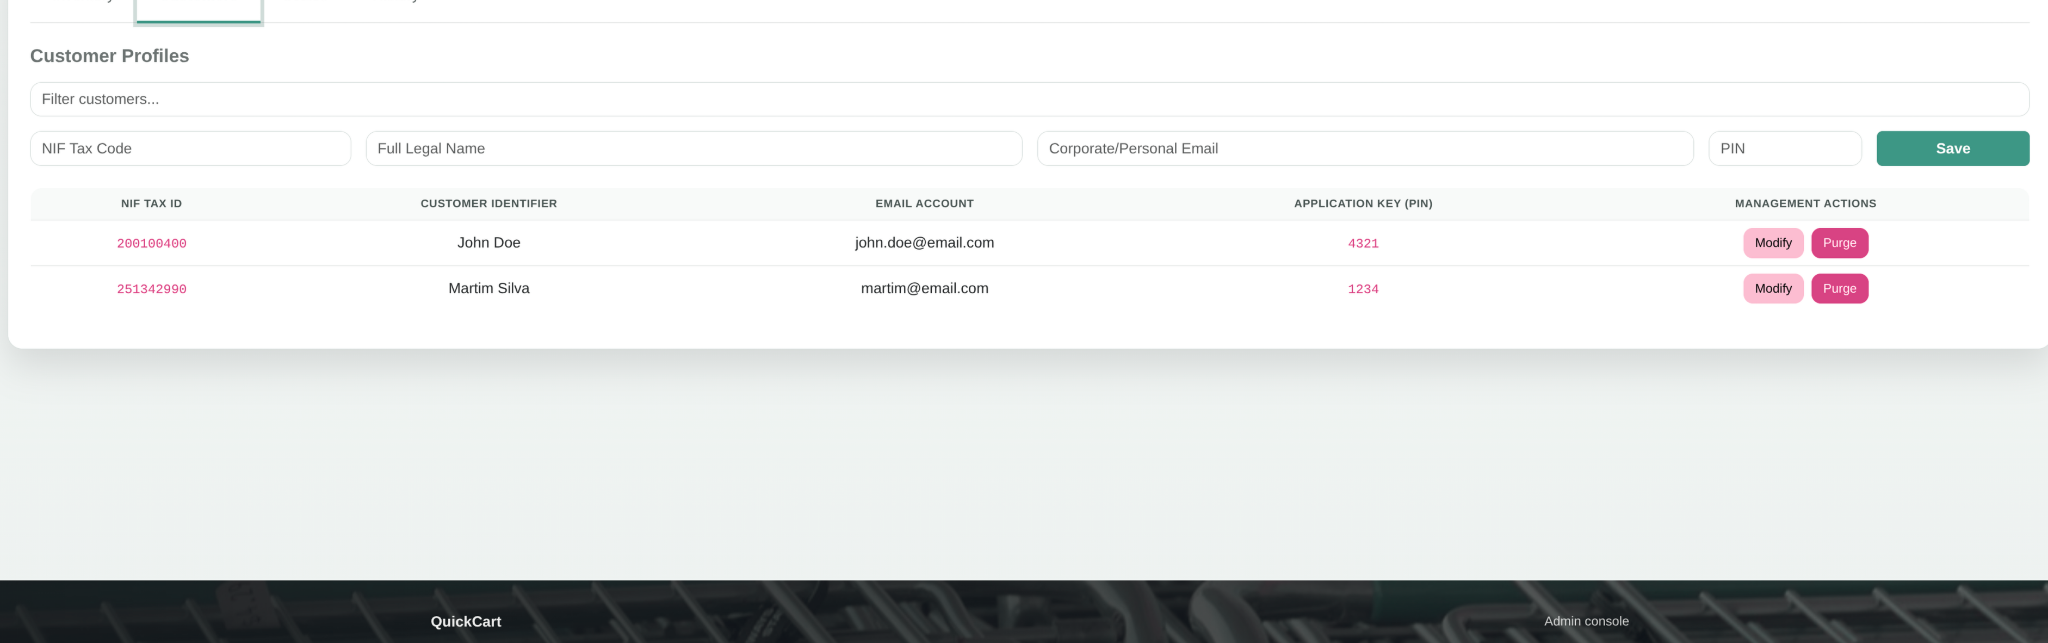
\includegraphics[width=\textwidth]{figures/admin_customers.png}
\caption{General-station customer management view.}
\label{fig:admin-customers}
\end{figure}

\begin{figure}[H]
\centering
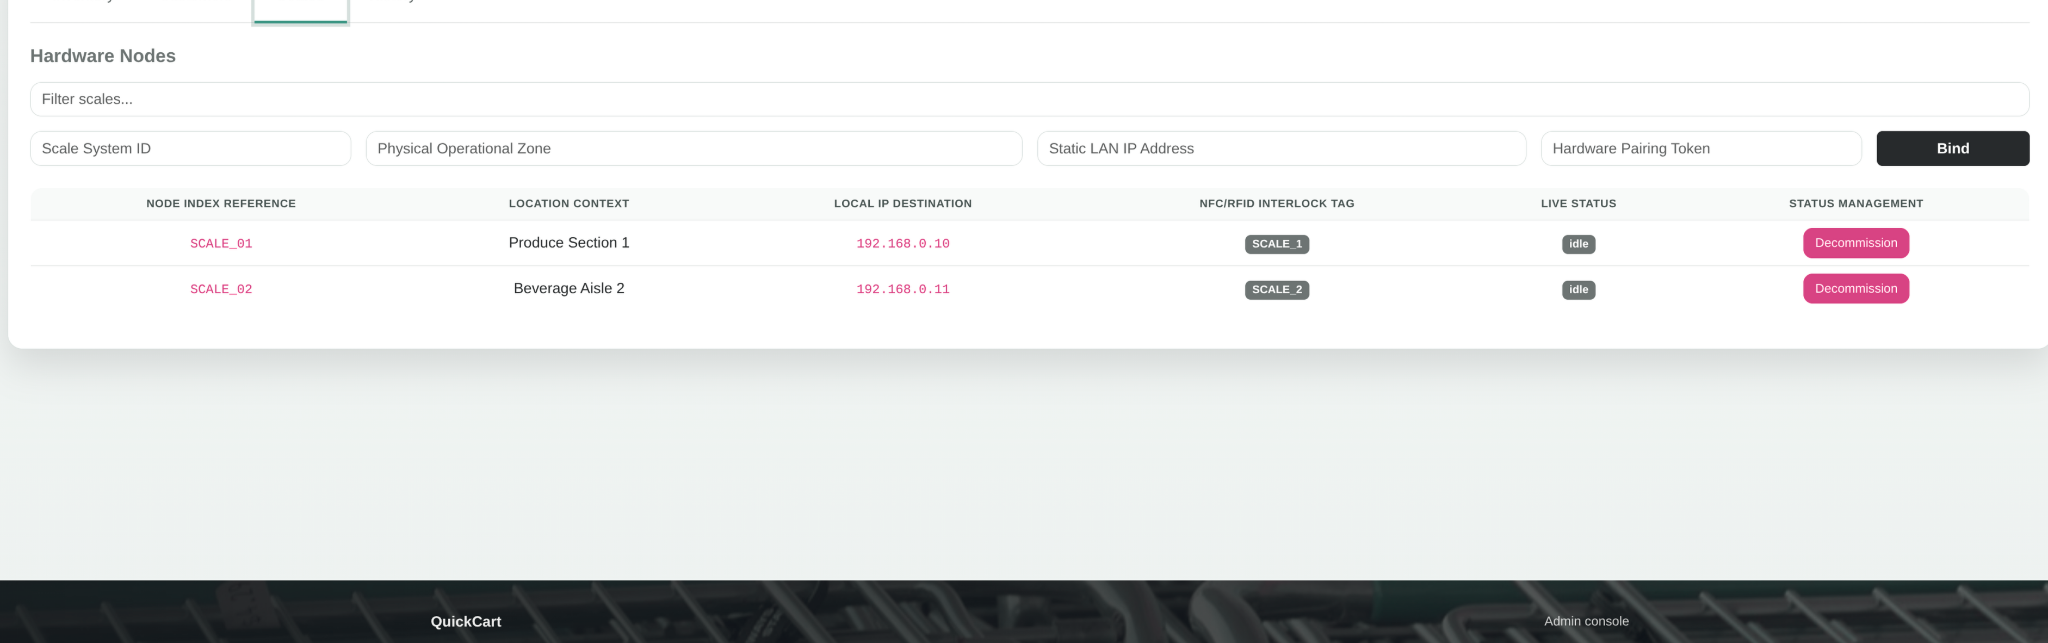
\includegraphics[width=\textwidth]{figures/admin_scales.png}
\caption{General-station scale-node management view, showing two registered cashier nodes and their pairing tags.}
\label{fig:admin-scales}
\end{figure}

% Replace this placeholder box with \includegraphics after capturing the final History view.
\begin{figure}[H]
\centering
\figureplaceholder{figures/admin\_history\_receipt.png}{4.5cm}
\caption{Archived receipt detail shown in the History panel of the central station.}
\label{fig:admin-history}
\end{figure}



\subsection{Integration Test Environment}

In addition to the final physical validation, a software-in-the-loop environment was used to verify the communication and application logic on a single development computer. This environment comprised:
\begin{itemize}
    \item the Raspberry Pi server application executed locally;
    \item a local MQTT broker;
    \item one or two Python mock scale processes that publish RFID and weight readings using the same message flow expected from physical cashier nodes;
    \item a mock Android client capable of authenticating, associating with a scale, receiving real-time cart updates and storing benchmark measurements;
    \item the real Android application when testing the user interface and network connection to the server.
\end{itemize}

This environment validates application-level integration and the distribution of sessions across scales and clients. Its measured timings are reported separately from the physical RFID and load-cell validation results.

\section{Analysis and Evaluation}
\label{sec:analysis-evaluation}

\subsection{Functional Evaluation}

Functional tests were executed across the complete application workflow, beginning with customer authentication and scale pairing, followed by product acquisition, cart update, checkout and receipt archival. Table~\ref{tab:functional-evaluation} summarises the observed system response.

\begin{table}[H]
\centering
\caption{Functional validation of the implemented workflow.}
\label{tab:functional-evaluation}
\begin{tabularx}{\textwidth}{@{}p{0.32\textwidth}Y p{0.15\textwidth}@{}}
\toprule
\textbf{Test Scenario} & \textbf{Observed Result} & \textbf{Status} \\
\midrule
Authentication and session creation & A registered customer successfully authenticated in the Android application and received a dedicated shopping-list session. & Passed \\
Scale selection by tag & Reading the scale pairing tag associated the smartphone session with the correct cashier node after the tare acknowledgement. & Passed \\
Weight-priced product & The server identified the product, applied the database price per kilogram and delivered the calculated line item to the mobile cart. & Passed \\
Empty-scale weighted product & The product remained pending until a valid weight was acquired, while the mobile client received a waiting-for-weight notice. & Passed \\
Unit-priced product & The fixed per-item price was applied independently of the informational measured mass. & Passed \\
Checkout and receipt archive & The active shopping list was cleared and stored as one grouped receipt in the central archive. & Passed \\
General station monitoring & The dashboard displayed catalogue data, registered customers, scale nodes, runtime status and archived purchases. & Passed \\
Two independent sessions & Products read on each scale were routed only to the smartphone associated with that cashier node. & Passed \\
\bottomrule
\end{tabularx}
\end{table}

\subsection{Software Communication Benchmark}

Before the final hardware measurement campaign, the server processing and communication logic was validated with simulated scale events transmitted through the same MQTT and Socket.IO integration path used by the implementation. The execution log contained thirteen completed product events and included the pending-weight condition for a weighted product detected before a positive mass reading was available.

\begin{table}[H]
\centering
\caption{Software-in-the-loop server processing benchmark.}
\label{tab:preliminary}
\begin{tabular}{@{}lr@{}}
\toprule
\textbf{Metric} & \textbf{Result} \\
\midrule
Completed product events recorded & 13 \\
Mean server processing time & 7.0 ms \\
Minimum server processing time & 6 ms \\
Maximum server processing time & 8 ms \\
Events below 2000 ms processing threshold & 13/13 \\
Pending-weight behaviour observed & Yes \\
\bottomrule
\end{tabular}
\end{table}

These preliminary measurements were used to confirm the correctness and responsiveness of the software pipeline prior to physical validation.

\subsection{Physical Timing Evaluation}

The final physical evaluation was conducted using the assembled Raspberry Pi general station, two cashier nodes and two Android smartphones connected to the same local network. RFID identification, weight stabilisation and visible list propagation were measured separately so that each time-bound requirement could be evaluated directly.

\begin{figure}[H]
\centering
\begin{subfigure}[t]{0.47\textwidth}
\centering
\figureplaceholder{figures/physical\_setup\_overview.png}{4.4cm}
\caption{Complete assembled setup used in evaluation.}
\end{subfigure}
\hfill
\begin{subfigure}[t]{0.47\textwidth}
\centering
\figureplaceholder{figures/cashier\_node\_wiring.png}{4.4cm}
\caption{Cashier acquisition node and wiring.}
\end{subfigure}
\caption{Physical hardware used during final validation.}
\label{fig:physical-setup}
\end{figure}

\begin{table}[H]
\centering
\small
\caption{Physical timing results for individual cashier-node operation.}
\label{tab:physical-individual}
\begin{tabularx}{\textwidth}{@{}p{0.20\textwidth}p{0.20\textwidth}p{0.20\textwidth}p{0.22\textwidth}Y@{}}
\toprule
\textbf{Scale} & \textbf{RFID Time} & \textbf{Weight Time} & \textbf{Update Time} & \textbf{Result} \\
\midrule
SCALE\_01 & \blankms & \blankms & \blankms & Passed \\
SCALE\_02 & \blankms & \blankms & \blankms & Passed \\
\bottomrule
\end{tabularx}
\end{table}



The measured values confirmed that product identification, weight stabilization and list updates remained within the required two-second bounds. In addition to standard reads, the empty-scale case was tested for a weight-priced item: the system postponed the line-item calculation until a stable mass became available and notified the customer through the mobile interface.

\begin{table}[H]
\centering
\small
\caption{Behavioural validation of pricing and checkout handling.}
\label{tab:physical-behaviour}
\begin{tabularx}{\textwidth}{@{}p{0.30\textwidth}Y p{0.16\textwidth}@{}}
\toprule
\textbf{Scenario} & \textbf{Observed Behaviour} & \textbf{Result} \\
\midrule
Bulk product with empty scale & A waiting-for-weight notification was displayed and no premature charge was inserted in the cart. & Passed \\
Bulk product with stable mass & The charged amount was calculated from measured kilograms and the centrally stored kilogram price. & Passed \\
Unit-priced product & The fixed unit price was used and the measured mass remained informational. & Passed \\
Checkout/reset & The active list was cleared and a complete archived receipt was generated on the central station. & Passed \\
\bottomrule
\end{tabularx}
\end{table}

\subsection{Concurrent Two-Station Evaluation}

A simultaneous-use test was performed with Smartphone A assigned to \texttt{SCALE\_01} and Smartphone B assigned to \texttt{SCALE\_02}. Product reads were generated at both cashier nodes within the same test interval. Both carts remained independent: each Android client received only the products acquired at its selected scale, while the general station displayed both active shopping lists concurrently.

\begin{figure}[H]
\centering
\figureplaceholder{figures/two\_phones\_two\_scales.png}{5.2cm}
\caption{Concurrent two-scale and two-smartphone physical validation.}
\label{fig:concurrent-physical}
\end{figure}

\begin{table}[H]
\centering
\caption{Concurrent two-scale/two-smartphone validation results.}
\label{tab:physical-concurrent}
\begin{tabularx}{\textwidth}{@{}p{0.31\textwidth}Y p{0.17\textwidth}@{}}
\toprule
\textbf{Check} & \textbf{Observed Result} & \textbf{Status} \\
\midrule
Smartphone A / SCALE\_01 routing & Only items acquired by SCALE\_01 were received by Smartphone A. & Passed \\
Smartphone B / SCALE\_02 routing & Only items acquired by SCALE\_02 were received by Smartphone B. & Passed \\
General-station live view & Both active lists were simultaneously visible at the central station. & Passed \\
Receipt archive isolation & Completing one list did not modify or clear the other active list. & Passed \\
\bottomrule
\end{tabularx}
\end{table}

\subsection{Final Requirement Compliance}

Table~\ref{tab:compliance} consolidates the completed functional and temporal validation. Numerical entries left blank are to be populated directly from the final physical-test measurement log.

\begin{table}[H]
\centering
\caption{Final compliance summary for the completed system.}
\label{tab:compliance}
\begin{tabularx}{\textwidth}{@{}p{0.38\textwidth}p{0.18\textwidth}Y p{0.14\textwidth}@{}}
\toprule
\textbf{Requirement} & \textbf{Target} & \textbf{Measured Result} & \textbf{Status} \\
\midrule
Product RFID identification & $< 2$ s & \blankms & Passed \\
Weight reading and stabilisation & $< 2$ s &  \blankms & Passed \\
Product visible on smartphone list & $< 2$ s &  \blankms & Passed \\
Product visible on general station & $< 2$ s & \blankms & Passed \\
Two independent scales/identifiers & 2 nodes & SCALE\_01 and SCALE\_02 operated concurrently. & Passed \\
Two independent Android clients & 2 clients & Two isolated shopping-list sessions were maintained. & Passed \\
Completed lists moved to archive & Required & Grouped receipt history recorded at checkout. & Passed \\
\bottomrule
\end{tabularx}
\end{table}

The final validation campaign comprised \blankvalue{1.4cm} measured product acquisitions per scale. The greatest recorded end-to-end update delay was \blankms, and all readings satisfied the maximum allowed delay of two seconds. No cross-routing of shopping-list products was observed during concurrent two-client operation.

\subsection{Engineering Observations}

The implemented architecture centralises session state, pricing rules and receipt archival at the Raspberry Pi, which prevents temporary client disconnection from discarding an active list. Separating fixed unit pricing from kilogram-based pricing also permits products to be handled according to their commercial model, while the pending-weight notification avoids incorrectly charging a weighted product before a stable measurement has been obtained.

\section{Conclusion}

The Weighting Cashier system fulfils the intended distributed-checkout workflow. Two cashier nodes identify and weigh products, the Raspberry Pi maintains authenticated sessions and centrally stored price rules, the Android applications display shopping lists in real time, and completed lists are stored as grouped archived receipts at the general station.

The software communication benchmark established a low server processing overhead, with a mean processing time of 7.0 ms for the simulated events. In the final physical validation, the maximum RFID identification delay was \blankms, the maximum weight-acquisition delay was \blankms, and the maximum user-visible list propagation delay was \blankms. These results remained below the required two-second limit. The simultaneous two-scale/two-smartphone evaluation also confirmed independent cart routing and correct archive operation.

\appendix



\end{document}
